\chapter{Aufbau: Erweiterung und Bestimmung der Transmission }
\thispagestyle{fancy}

\section{Bestimmung der Transmission des UV Quarzglases}

Da die Messung der Anregungsleistungdichte erfolgt, bevor das Laserlicht die Probe durch das UV-Quarzglas im Kryostaten trifft, ist es wichtig den Transmissionsverlust zu bestimmen, um die realen Werte für die Anregungsleistungsdichte zu kennen (Die Anregungsleistungsdichte die bei der Probe ankommt). Der Kryostat besitzt vier Fenster, bestehend aus UV-Quarzglas, das besonders transparent im UV-Wellenlängen bereich ist. Durch diese Fenster dringt das Laserlicht in den Probenhalter ein. Von diesen Fenstern war und ist eines in dauerhaftem Gebrauch. Wie in Abb. [] zu sehen ist, weisen die Fenster aber mit der Anzahl der Pulse eine fortlaufende Abnutzung auf, so nimmt laut Hersteller durch Degradation die Transmission von 90 Prozent bis auf ca. 75 Prozent ab für eine Wellenlänge von 193 nm. 


Um nun den Transmissongrad zu bestimmen, wurde der Probenhalter aus dem Kryostat entfernt, damit das Laserlicht ungehindert durch zwei parallel liegende Fenster durchdringen kann, um so auch die Anregungsleistungsdichte des Laserlichtes nach durchdringen des letzten Fenster messen zu können. So konnte die Anregungsleistungsdichte vor dem Eintreten und nach dem Austreten in den Kryostaten bestimmt werden. 
Dies wurde einmal bei den parallel liegenden unbenutzten Fenstern gemacht. Davon ausgehend, dass beide Fenster, da unbenutzt, den gleichen Transmissionsgrad haben, kann darauf zurückgeschlossen werden, dass ein unbenutztes Fenster einen Transmissionsgrad von 59 Prozent aufweist, was um ca. 10 Prozent von der Herstellerangabe abweicht. 
Um den Transmissionsgrad des benutzten Fensters zu bestimmen, wurde die Transmission durch das benutzte Fenster und dem parallel liegenden unbenutzten Fenster gemessen. Mit dem Wissen, dass der Transmissionsgrad durch das unbenutzte Fensters bei 59 Prozent, kann die Transmission durch das benutzte Fenster auf 29 Prozent runtergerechnet werden. 
Davon ausgehend, dass die Transmission bei höheren Wellenlängen 90 Prozent beträgt, kann der Skalierungsfaktor auf 0,44 berechnet werden. 
\begin{figure}
    \centering
    \begin{subfigure}{0.5\textwidth}
      \centering
      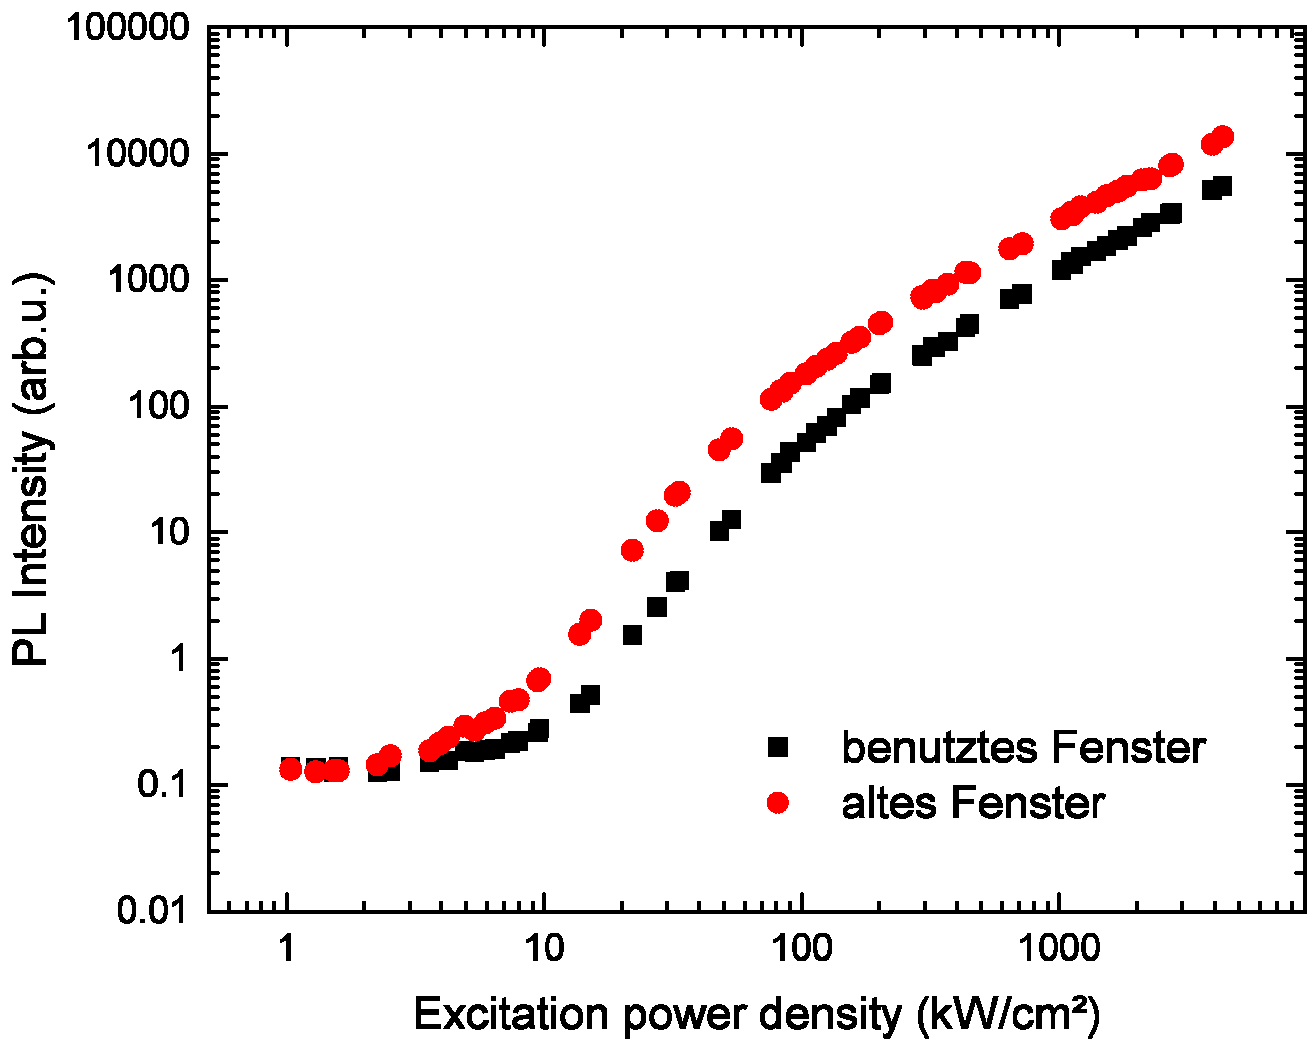
\includegraphics[width=0.9\linewidth]{Bilder/uvsilicavergleich.pdf}
      \caption{A subfigure}
      \label{fig:sub1}
    \end{subfigure}%
    \begin{subfigure}{0.5\textwidth}
      \centering
      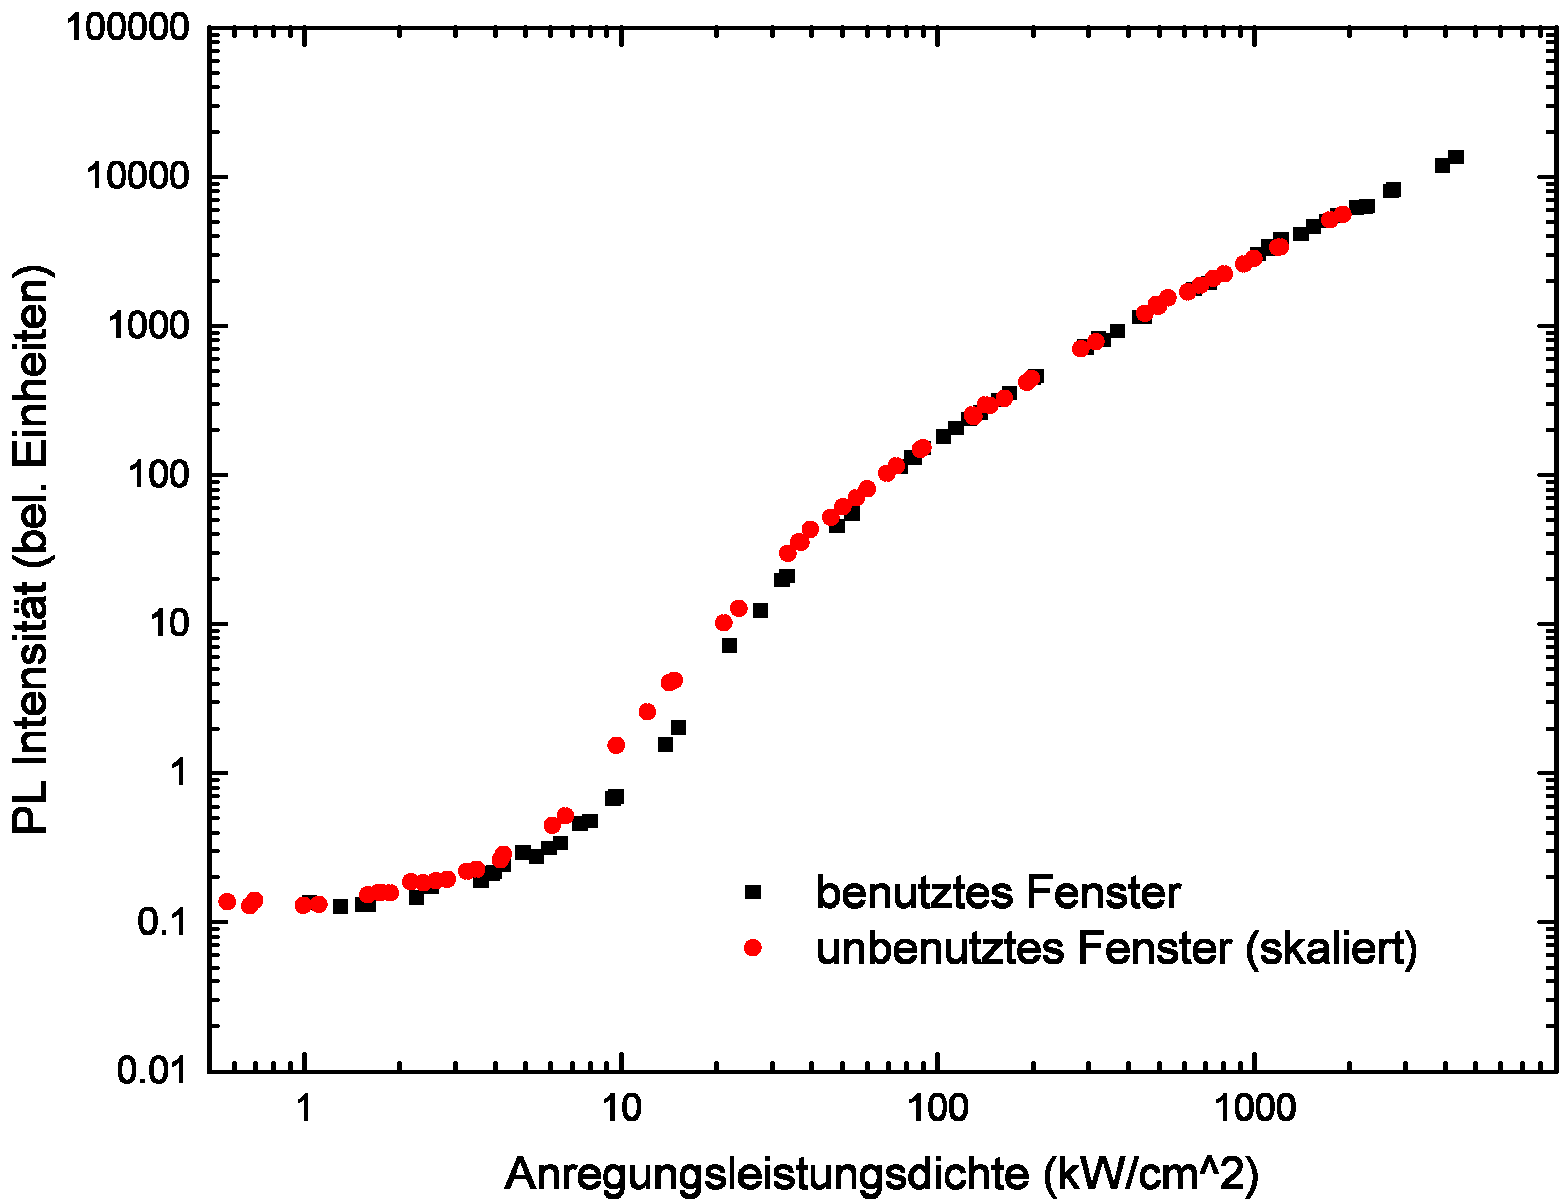
\includegraphics[width=0.9\linewidth]{Bilder/uvsilicaVergleichSkaliert.pdf}
      \caption{A subfigure}
      \label{fig:sub2}
    \end{subfigure}
    \caption{A figure with two subfigures}
    \label{fig:test}
    \end{figure}
